\documentclass[tikz,border=2pt]{standalone}
\usepackage{tikz}
\usetikzlibrary{arrows,positioning,shapes}
\begin{document}
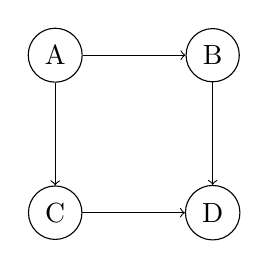
\begin{tikzpicture}[node distance=2cm]
  \node[circle,draw] (A) {A};
  \node[circle,draw] (B) [right of=A] {B};
  \node[circle,draw] (C) [below of=A] {C};
  \node[circle,draw] (D) [right of=C] {D};
  
  \draw[->] (A) -- (B);
  \draw[->] (A) -- (C);
  \draw[->] (B) -- (D);
  \draw[->] (C) -- (D);
\end{tikzpicture}
\end{document}
